% Options for packages loaded elsewhere
\PassOptionsToPackage{unicode}{hyperref}
\PassOptionsToPackage{hyphens}{url}
%
\documentclass[
]{article}
\usepackage{amsmath,amssymb}
\usepackage{lmodern}
\usepackage{iftex}
\ifPDFTeX
  \usepackage[T1]{fontenc}
  \usepackage[utf8]{inputenc}
  \usepackage{textcomp} % provide euro and other symbols
\else % if luatex or xetex
  \usepackage{unicode-math}
  \defaultfontfeatures{Scale=MatchLowercase}
  \defaultfontfeatures[\rmfamily]{Ligatures=TeX,Scale=1}
\fi
% Use upquote if available, for straight quotes in verbatim environments
\IfFileExists{upquote.sty}{\usepackage{upquote}}{}
\IfFileExists{microtype.sty}{% use microtype if available
  \usepackage[]{microtype}
  \UseMicrotypeSet[protrusion]{basicmath} % disable protrusion for tt fonts
}{}
\makeatletter
\@ifundefined{KOMAClassName}{% if non-KOMA class
  \IfFileExists{parskip.sty}{%
    \usepackage{parskip}
  }{% else
    \setlength{\parindent}{0pt}
    \setlength{\parskip}{6pt plus 2pt minus 1pt}}
}{% if KOMA class
  \KOMAoptions{parskip=half}}
\makeatother
\usepackage{xcolor}
\usepackage[margin=1in]{geometry}
\usepackage{graphicx}
\makeatletter
\def\maxwidth{\ifdim\Gin@nat@width>\linewidth\linewidth\else\Gin@nat@width\fi}
\def\maxheight{\ifdim\Gin@nat@height>\textheight\textheight\else\Gin@nat@height\fi}
\makeatother
% Scale images if necessary, so that they will not overflow the page
% margins by default, and it is still possible to overwrite the defaults
% using explicit options in \includegraphics[width, height, ...]{}
\setkeys{Gin}{width=\maxwidth,height=\maxheight,keepaspectratio}
% Set default figure placement to htbp
\makeatletter
\def\fps@figure{htbp}
\makeatother
\setlength{\emergencystretch}{3em} % prevent overfull lines
\providecommand{\tightlist}{%
  \setlength{\itemsep}{0pt}\setlength{\parskip}{0pt}}
\setcounter{secnumdepth}{-\maxdimen} % remove section numbering
\usepackage{booktabs}
\usepackage{longtable}
\usepackage{array}
\usepackage{multirow}
\usepackage{wrapfig}
\usepackage{float}
\usepackage{colortbl}
\usepackage{pdflscape}
\usepackage{tabu}
\usepackage{threeparttable}
\usepackage{threeparttablex}
\usepackage[normalem]{ulem}
\usepackage{makecell}
\usepackage{xcolor}
\ifLuaTeX
  \usepackage{selnolig}  % disable illegal ligatures
\fi
\IfFileExists{bookmark.sty}{\usepackage{bookmark}}{\usepackage{hyperref}}
\IfFileExists{xurl.sty}{\usepackage{xurl}}{} % add URL line breaks if available
\urlstyle{same} % disable monospaced font for URLs
\hypersetup{
  pdftitle={Research Assistantship - Data Collection},
  pdfauthor={Federico Vicentini},
  hidelinks,
  pdfcreator={LaTeX via pandoc}}

\title{Research Assistantship - Data Collection}
\author{Federico Vicentini}
\date{01/05/2023}

\begin{document}
\maketitle

\hypertarget{data-collection}{%
\section{DATA COLLECTION}\label{data-collection}}

\hypertarget{real-gdp-data}{%
\subsection{Real GDP Data}\label{real-gdp-data}}

\par

In this first part, we download nominal GDP data and GDP deflator data
from 1980 to 2020 and then we divide it into the 2 section (1980s and
2010s) in order to calculate means and thus compare it to the data we
got in the TTD Presentation.

\begin{verbatim}
## [1] 2.816635
\end{verbatim}

\begin{verbatim}
## [1] 3.813955
\end{verbatim}

\begin{verbatim}
## [1] 2.424288
\end{verbatim}

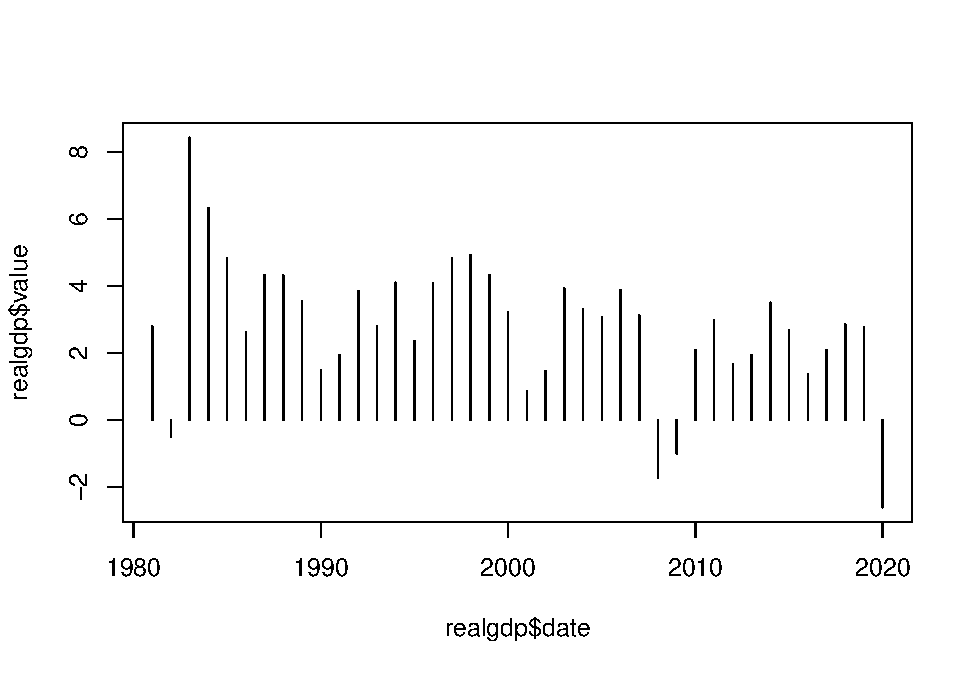
\includegraphics{datacollection_files/figure-latex/p1.1-1.pdf}
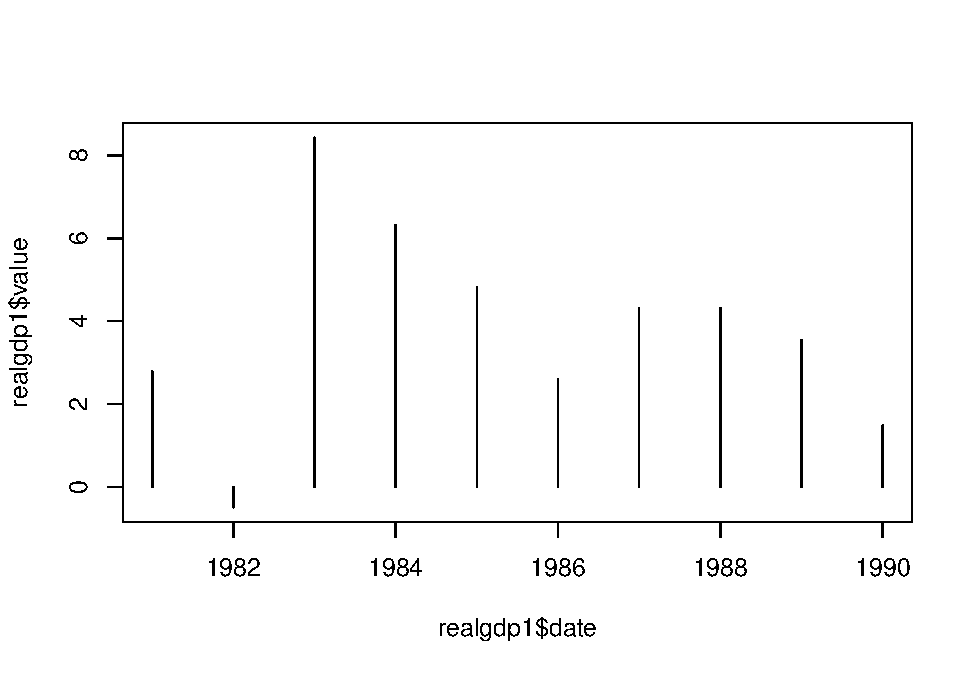
\includegraphics{datacollection_files/figure-latex/p1.1-2.pdf}
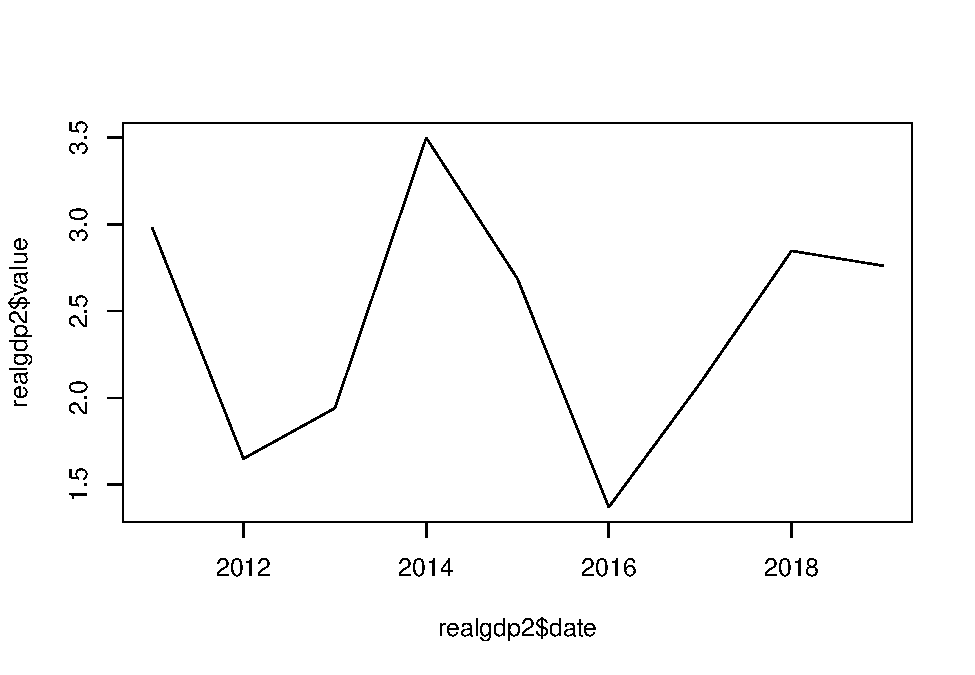
\includegraphics{datacollection_files/figure-latex/p1.1-3.pdf}

\hypertarget{labor-share-of-output}{%
\subsection{Labor Share of Output}\label{labor-share-of-output}}

\hypertarget{naive-labor-share}{%
\subsubsection{``Naive'' Labor Share}\label{naive-labor-share}}

First attmpt here is to download the laborshare timeseries from fred.
Howevere, this approach neglects some important aspects, such as the
role of self-employed workers and correction to value added in the forms
of indirect taxes and consumption of fixed capital.

\hypertarget{guerriero-index}{%
\subsubsection{Guerriero Index}\label{guerriero-index}}

This is precisely why I tried to replicate the laborshare measure
provided by Guerriero (2019), defined as:

\[LS6 = \frac{compensation\;of\;employees * 
\left(\frac{workforce-employers}{employees}\right)}
{value\;added-ind.\;taxes-fixed\;cap.\;cons.}\]

\includegraphics{datacollection_files/figure-latex/p2.1-1.pdf}

\begin{verbatim}
## 
## ############################################### 
## # Augmented Dickey-Fuller Test Unit Root Test # 
## ############################################### 
## 
## Test regression drift 
## 
## 
## Call:
## lm(formula = z.diff ~ z.lag.1 + 1 + z.diff.lag)
## 
## Residuals:
##        Min         1Q     Median         3Q        Max 
## -7.085e+09 -2.684e+08  4.544e+08  9.162e+08  6.895e+09 
## 
## Coefficients:
##               Estimate Std. Error t value Pr(>|t|)  
## (Intercept)  4.821e+08  1.063e+09   0.454   0.6588  
## z.lag.1     -5.694e-01  2.167e-01  -2.627   0.0235 *
## z.diff.lag   6.012e-01  2.718e-01   2.212   0.0491 *
## ---
## Signif. codes:  0 '***' 0.001 '**' 0.01 '*' 0.05 '.' 0.1 ' ' 1
## 
## Residual standard error: 3.916e+09 on 11 degrees of freedom
## Multiple R-squared:  0.4223, Adjusted R-squared:  0.3173 
## F-statistic: 4.021 on 2 and 11 DF,  p-value: 0.04889
## 
## 
## Value of test-statistic is: -2.6273 3.452 
## 
## Critical values for test statistics: 
##       1pct  5pct 10pct
## tau2 -3.75 -3.00 -2.63
## phi1  7.88  5.18  4.12
## 
## 
## ===============================================
##                         Dependent variable:    
##                     ---------------------------
##                                 s1             
## -----------------------------------------------
## lag_s1                       1.072***          
##                               (0.021)          
##                                                
## Constant                -8,250,169,233.000     
##                         (6,753,307,947.000)    
##                                                
## -----------------------------------------------
## Observations                    16             
## R2                             0.995           
## Adjusted R2                    0.994           
## Residual Std. Error 5,773,614,796.000 (df = 14)
## F Statistic          2,533.752*** (df = 1; 14) 
## ===============================================
## Note:               *p<0.1; **p<0.05; ***p<0.01
## 
## ############################################### 
## # Augmented Dickey-Fuller Test Unit Root Test # 
## ############################################### 
## 
## Test regression drift 
## 
## 
## Call:
## lm(formula = z.diff ~ z.lag.1 + 1 + z.diff.lag)
## 
## Residuals:
##        Min         1Q     Median         3Q        Max 
## -2.782e+09 -1.537e+09 -3.670e+08  1.329e+09  5.376e+09 
## 
## Coefficients:
##               Estimate Std. Error t value Pr(>|t|)  
## (Intercept)  3.979e+08  6.768e+08   0.588   0.5685  
## z.lag.1     -6.951e-01  2.334e-01  -2.978   0.0126 *
## z.diff.lag   6.937e-01  2.924e-01   2.372   0.0370 *
## ---
## Signif. codes:  0 '***' 0.001 '**' 0.01 '*' 0.05 '.' 0.1 ' ' 1
## 
## Residual standard error: 2.481e+09 on 11 degrees of freedom
## Multiple R-squared:  0.4666, Adjusted R-squared:  0.3697 
## F-statistic: 4.812 on 2 and 11 DF,  p-value: 0.03152
## 
## 
## Value of test-statistic is: -2.9778 4.4372 
## 
## Critical values for test statistics: 
##       1pct  5pct 10pct
## tau2 -3.75 -3.00 -2.63
## phi1  7.88  5.18  4.12
## 
## 
## ===============================================
##                         Dependent variable:    
##                     ---------------------------
##                                 s2             
## -----------------------------------------------
## lag_s2                       1.035***          
##                               (0.020)          
##                                                
## Constant                 3,403,259,047.000     
##                         (3,258,937,291.000)    
##                                                
## -----------------------------------------------
## Observations                    16             
## R2                             0.995           
## Adjusted R2                    0.994           
## Residual Std. Error 3,504,860,995.000 (df = 14)
## F Statistic          2,681.792*** (df = 1; 14) 
## ===============================================
## Note:               *p<0.1; **p<0.05; ***p<0.01
## 
## ===============================================
##                         Dependent variable:    
##                     ---------------------------
##                                 s1             
## -----------------------------------------------
## s2                           1.850***          
##                               (0.208)          
##                                                
## Constant                -2,522,381,155.000     
##                         (1,997,242,452.000)    
##                                                
## -----------------------------------------------
## Observations                    16             
## R2                             0.850           
## Adjusted R2                    0.839           
## Residual Std. Error 3,007,268,669.000 (df = 14)
## F Statistic           79.400*** (df = 1; 14)   
## ===============================================
## Note:               *p<0.1; **p<0.05; ***p<0.01
## 
## ====
## TRUE
## ----
\end{verbatim}

\includegraphics{datacollection_files/figure-latex/p2.1-2.pdf}

\begin{verbatim}
## 
## ############################################### 
## # Augmented Dickey-Fuller Test Unit Root Test # 
## ############################################### 
## 
## Test regression drift 
## 
## 
## Call:
## lm(formula = z.diff ~ z.lag.1 + 1 + z.diff.lag)
## 
## Residuals:
##        Min         1Q     Median         3Q        Max 
## -3.397e+10 -4.067e+07  2.066e+09  7.209e+09  1.795e+10 
## 
## Coefficients:
##               Estimate Std. Error t value Pr(>|t|)
## (Intercept) -8.930e+08  4.250e+09  -0.210    0.837
## z.lag.1     -2.202e-01  2.826e-01  -0.779    0.452
## z.diff.lag   3.626e-01  3.698e-01   0.980    0.348
## 
## Residual standard error: 1.491e+10 on 11 degrees of freedom
## Multiple R-squared:  0.107,  Adjusted R-squared:  -0.05531 
## F-statistic: 0.6593 on 2 and 11 DF,  p-value: 0.5365
## 
## 
## Value of test-statistic is: -0.7791 0.4277 
## 
## Critical values for test statistics: 
##       1pct  5pct 10pct
## tau2 -3.75 -3.00 -2.63
## phi1  7.88  5.18  4.12
## 
## 
## ================================================
##                         Dependent variable:     
##                     ----------------------------
##                                  s1             
## ------------------------------------------------
## lag_s1                        1.022***          
##                               (0.016)           
##                                                 
## Constant                 32,300,824,321.000     
##                         (23,705,657,522.000)    
##                                                 
## ------------------------------------------------
## Observations                     16             
## R2                             0.997            
## Adjusted R2                    0.996            
## Residual Std. Error 21,046,319,844.000 (df = 14)
## F Statistic          4,139.821*** (df = 1; 14)  
## ================================================
## Note:                *p<0.1; **p<0.05; ***p<0.01
## 
## ############################################### 
## # Augmented Dickey-Fuller Test Unit Root Test # 
## ############################################### 
## 
## Test regression drift 
## 
## 
## Call:
## lm(formula = z.diff ~ z.lag.1 + 1 + z.diff.lag)
## 
## Residuals:
##        Min         1Q     Median         3Q        Max 
## -2.172e+10 -4.903e+09 -1.365e+09  9.736e+09  1.852e+10 
## 
## Coefficients:
##               Estimate Std. Error t value Pr(>|t|)
## (Intercept)  1.186e+07  3.786e+09   0.003    0.998
## z.lag.1     -3.078e-01  2.432e-01  -1.266    0.232
## z.diff.lag   4.854e-01  3.129e-01   1.551    0.149
## 
## Residual standard error: 1.355e+10 on 11 degrees of freedom
## Multiple R-squared:  0.2093, Adjusted R-squared:  0.06558 
## F-statistic: 1.456 on 2 and 11 DF,  p-value: 0.2748
## 
## 
## Value of test-statistic is: -1.2659 0.8741 
## 
## Critical values for test statistics: 
##       1pct  5pct 10pct
## tau2 -3.75 -3.00 -2.63
## phi1  7.88  5.18  4.12
## 
## 
## ================================================
##                         Dependent variable:     
##                     ----------------------------
##                                  s2             
## ------------------------------------------------
## lag_s2                        1.019***          
##                               (0.017)           
##                                                 
## Constant                 34,748,116,629.000     
##                         (22,551,045,966.000)    
##                                                 
## ------------------------------------------------
## Observations                     16             
## R2                             0.996            
## Adjusted R2                    0.996            
## Residual Std. Error 20,958,000,953.000 (df = 14)
## F Statistic          3,560.294*** (df = 1; 14)  
## ================================================
## Note:                *p<0.1; **p<0.05; ***p<0.01
## 
## ===============================================
##                         Dependent variable:    
##                     ---------------------------
##                                 s1             
## -----------------------------------------------
## s2                           1.000***          
##                               (0.063)          
##                                                
## Constant                 5,325,487,495.000     
##                         (3,959,430,158.000)    
##                                                
## -----------------------------------------------
## Observations                    16             
## R2                             0.947           
## Adjusted R2                    0.944           
## Residual Std. Error 5,157,300,357.000 (df = 14)
## F Statistic           251.972*** (df = 1; 14)  
## ===============================================
## Note:               *p<0.1; **p<0.05; ***p<0.01
## 
## ====
## TRUE
## ----
\end{verbatim}

\includegraphics{datacollection_files/figure-latex/p2.1-3.pdf}

\begin{verbatim}
## 
## ############################################### 
## # Augmented Dickey-Fuller Test Unit Root Test # 
## ############################################### 
## 
## Test regression drift 
## 
## 
## Call:
## lm(formula = z.diff ~ z.lag.1 + 1 + z.diff.lag)
## 
## Residuals:
##        Min         1Q     Median         3Q        Max 
## -4.239e+10  6.862e+08  2.398e+09  7.659e+09  1.728e+10 
## 
## Coefficients:
##               Estimate Std. Error t value Pr(>|t|)
## (Intercept) -9.729e+08  4.651e+09  -0.209    0.838
## z.lag.1     -2.576e-01  3.465e-01  -0.743    0.473
## z.diff.lag   2.745e-01  4.382e-01   0.626    0.544
## 
## Residual standard error: 1.583e+10 on 11 degrees of freedom
## Multiple R-squared:  0.07293,    Adjusted R-squared:  -0.09562 
## F-statistic: 0.4327 on 2 and 11 DF,  p-value: 0.6593
## 
## 
## Value of test-statistic is: -0.7435 0.4192 
## 
## Critical values for test statistics: 
##       1pct  5pct 10pct
## tau2 -3.75 -3.00 -2.63
## phi1  7.88  5.18  4.12
## 
## 
## ================================================
##                         Dependent variable:     
##                     ----------------------------
##                                  s1             
## ------------------------------------------------
## lag_s1                        1.008***          
##                               (0.018)           
##                                                 
## Constant                43,038,499,984.000*     
##                         (21,355,529,797.000)    
##                                                 
## ------------------------------------------------
## Observations                     16             
## R2                             0.996            
## Adjusted R2                    0.995            
## Residual Std. Error 19,746,841,918.000 (df = 14)
## F Statistic          3,152.096*** (df = 1; 14)  
## ================================================
## Note:                *p<0.1; **p<0.05; ***p<0.01
## 
## ############################################### 
## # Augmented Dickey-Fuller Test Unit Root Test # 
## ############################################### 
## 
## Test regression drift 
## 
## 
## Call:
## lm(formula = z.diff ~ z.lag.1 + 1 + z.diff.lag)
## 
## Residuals:
##        Min         1Q     Median         3Q        Max 
## -2.391e+10 -3.434e+09  4.800e+08  8.329e+09  1.863e+10 
## 
## Coefficients:
##               Estimate Std. Error t value Pr(>|t|)
## (Intercept) -2.490e+08  3.880e+09  -0.064    0.950
## z.lag.1     -3.145e-01  2.665e-01  -1.180    0.263
## z.diff.lag   4.504e-01  3.290e-01   1.369    0.198
## 
## Residual standard error: 1.385e+10 on 11 degrees of freedom
## Multiple R-squared:  0.181,  Adjusted R-squared:  0.03208 
## F-statistic: 1.215 on 2 and 11 DF,  p-value: 0.3335
## 
## 
## Value of test-statistic is: -1.1801 0.7913 
## 
## Critical values for test statistics: 
##       1pct  5pct 10pct
## tau2 -3.75 -3.00 -2.63
## phi1  7.88  5.18  4.12
## 
## 
## ================================================
##                         Dependent variable:     
##                     ----------------------------
##                                  s2             
## ------------------------------------------------
## lag_s2                        1.017***          
##                               (0.018)           
##                                                 
## Constant                 33,117,178,138.000     
##                         (21,304,826,462.000)    
##                                                 
## ------------------------------------------------
## Observations                     16             
## R2                             0.996            
## Adjusted R2                    0.995            
## Residual Std. Error 19,892,178,980.000 (df = 14)
## F Statistic          3,106.851*** (df = 1; 14)  
## ================================================
## Note:                *p<0.1; **p<0.05; ***p<0.01
## 
## ===============================================
##                         Dependent variable:    
##                     ---------------------------
##                                 s1             
## -----------------------------------------------
## s2                           0.922***          
##                               (0.081)          
##                                                
## Constant                 4,308,912,458.000     
##                         (4,532,028,663.000)    
##                                                
## -----------------------------------------------
## Observations                    16             
## R2                             0.902           
## Adjusted R2                    0.895           
## Residual Std. Error 6,233,996,940.000 (df = 14)
## F Statistic           128.582*** (df = 1; 14)  
## ===============================================
## Note:               *p<0.1; **p<0.05; ***p<0.01
## 
## ====
## TRUE
## ----
\end{verbatim}

\includegraphics{datacollection_files/figure-latex/p2.1-4.pdf}

\begin{verbatim}
## 
## ############################################### 
## # Augmented Dickey-Fuller Test Unit Root Test # 
## ############################################### 
## 
## Test regression drift 
## 
## 
## Call:
## lm(formula = z.diff ~ z.lag.1 + 1 + z.diff.lag)
## 
## Residuals:
##        Min         1Q     Median         3Q        Max 
## -5.572e+10 -8.674e+09  1.043e+09  2.153e+10  2.983e+10 
## 
## Coefficients:
##               Estimate Std. Error t value Pr(>|t|)  
## (Intercept)  9.671e+08  6.884e+09   0.140   0.8908  
## z.lag.1     -6.986e-01  3.600e-01  -1.941   0.0783 .
## z.diff.lag  -2.032e-02  3.002e-01  -0.068   0.9472  
## ---
## Signif. codes:  0 '***' 0.001 '**' 0.01 '*' 0.05 '.' 0.1 ' ' 1
## 
## Residual standard error: 2.572e+10 on 11 degrees of freedom
## Multiple R-squared:  0.3562, Adjusted R-squared:  0.2391 
## F-statistic: 3.043 on 2 and 11 DF,  p-value: 0.08876
## 
## 
## Value of test-statistic is: -1.9407 1.8976 
## 
## Critical values for test statistics: 
##       1pct  5pct 10pct
## tau2 -3.75 -3.00 -2.63
## phi1  7.88  5.18  4.12
## 
## 
## ================================================
##                         Dependent variable:     
##                     ----------------------------
##                                  s1             
## ------------------------------------------------
## lag_s1                        0.990***          
##                               (0.036)           
##                                                 
## Constant                 40,159,652,434.000     
##                         (27,944,128,837.000)    
##                                                 
## ------------------------------------------------
## Observations                     16             
## R2                             0.982            
## Adjusted R2                    0.981            
## Residual Std. Error 24,070,285,996.000 (df = 14)
## F Statistic           776.524*** (df = 1; 14)   
## ================================================
## Note:                *p<0.1; **p<0.05; ***p<0.01
## 
## ############################################### 
## # Augmented Dickey-Fuller Test Unit Root Test # 
## ############################################### 
## 
## Test regression drift 
## 
## 
## Call:
## lm(formula = z.diff ~ z.lag.1 + 1 + z.diff.lag)
## 
## Residuals:
##        Min         1Q     Median         3Q        Max 
## -4.862e+10 -8.325e+09  9.378e+07  1.616e+10  2.844e+10 
## 
## Coefficients:
##               Estimate Std. Error t value Pr(>|t|)  
## (Intercept)  9.020e+08  6.401e+09   0.141   0.8905  
## z.lag.1     -7.291e-01  3.650e-01  -1.998   0.0711 .
## z.diff.lag  -1.761e-03  3.001e-01  -0.006   0.9954  
## ---
## Signif. codes:  0 '***' 0.001 '**' 0.01 '*' 0.05 '.' 0.1 ' ' 1
## 
## Residual standard error: 2.393e+10 on 11 degrees of freedom
## Multiple R-squared:  0.3632, Adjusted R-squared:  0.2475 
## F-statistic: 3.137 on 2 and 11 DF,  p-value: 0.08353
## 
## 
## Value of test-statistic is: -1.9978 2.0112 
## 
## Critical values for test statistics: 
##       1pct  5pct 10pct
## tau2 -3.75 -3.00 -2.63
## phi1  7.88  5.18  4.12
## 
## 
## ================================================
##                         Dependent variable:     
##                     ----------------------------
##                                  s2             
## ------------------------------------------------
## lag_s2                        0.991***          
##                               (0.034)           
##                                                 
## Constant                 38,847,511,824.000     
##                         (26,360,021,209.000)    
##                                                 
## ------------------------------------------------
## Observations                     16             
## R2                             0.984            
## Adjusted R2                    0.983            
## Residual Std. Error 22,264,324,356.000 (df = 14)
## F Statistic           864.627*** (df = 1; 14)   
## ================================================
## Note:                *p<0.1; **p<0.05; ***p<0.01
## 
## ===============================================
##                         Dependent variable:    
##                     ---------------------------
##                                 s1             
## -----------------------------------------------
## s2                           1.073***          
##                               (0.037)          
##                                                
## Constant                -1,864,883,147.000     
##                         (1,411,916,548.000)    
##                                                
## -----------------------------------------------
## Observations                    16             
## R2                             0.984           
## Adjusted R2                    0.983           
## Residual Std. Error 3,080,914,350.000 (df = 14)
## F Statistic           845.298*** (df = 1; 14)  
## ===============================================
## Note:               *p<0.1; **p<0.05; ***p<0.01
## 
## ====
## TRUE
## ----
\end{verbatim}

\includegraphics{datacollection_files/figure-latex/p2.1-5.pdf}

\end{document}
